%%%%%%%%%%%%%%%%%%%%%%%%%%%%%%%%%%%%%%%%%%%%%%%%%%%%%%%%%%%%%%%%%%%%%%%%
%%%%%%%%%%%%%%%%%%%%%% Simple LaTeX CV Template %%%%%%%%%%%%%%%%%%%%%%%%
%%%%%%%%%%%%%%%%%%%%%%%%%%%%%%%%%%%%%%%%%%%%%%%%%%%%%%%%%%%%%%%%%%%%%%%%

%%%%%%%%%%%%%%%%%%%%%%%%%%%%%%%%%%%%%%%%%%%%%%%%%%%%%%%%%%%%%%%%%%%%%%%%
%% NOTE: If you find that it says                                     %%
%%                                                                    %%
%%                           1 of ??                                  %%
%%                                                                    %%
%% at the bottom of your first page, this means that the AUX file     %%
%% was not available when you ran LaTeX on this source. Simply RERUN  %%
%% LaTeX to get the ``??'' replaced with the number of the last page  %%
%% of the document. The AUX file will be generated on the first run   %%
%% of LaTeX and used on the second run to fill in all of the          %%
%% references.                                                        %%
%%%%%%%%%%%%%%%%%%%%%%%%%%%%%%%%%%%%%%%%%%%%%%%%%%%%%%%%%%%%%%%%%%%%%%%%

%%%%%%%%%%%%%%%%%%%%%%%%%%%% Document Setup %%%%%%%%%%%%%%%%%%%%%%%%%%%%

% Don't like 10pt? Try 11pt or 12pt
\documentclass[10pt]{article}

% This is a helpful package that puts math inside length specifications
\usepackage{calc, graphicx}
\usepackage{polski}
\usepackage[utf8]{inputenc}
\usepackage{multirow}

\usepackage{hyperref}

\hypersetup{
    bookmarks=true,         % show bookmarks bar?
    unicode=false,          % non-Latin characters in Acrobat’s bookmarks
    pdftoolbar=true,        % show Acrobat’s toolbar?
    pdfmenubar=true,        % show Acrobat’s menu?
    pdffitwindow=false,     % window fit to page when opened
    pdfstartview={FitH},    % fits the width of the page to the window
    pdftitle={My title},    % title
    pdfauthor={Author},     % author
    pdfsubject={Subject},   % subject of the document
    pdfcreator={Creator},   % creator of the document
    pdfproducer={Producer}, % producer of the document
    pdfkeywords={keywords}, % list of keywords
    pdfnewwindow=true,      % links in new window
    colorlinks=true,       % false: boxed links; true: colored links
    linkcolor=red,          % color of internal links
    citecolor=green,        % color of links to bibliography
    filecolor=magenta,      % color of file links
    urlcolor=black          % color of external links
}


% Simpler bibsection for CV sections
% (thanks to natbib for inspiration)
\makeatletter
\newlength{\bibhang}
\setlength{\bibhang}{1em}
\newlength{\bibsep}
 {\@listi \global\bibsep\itemsep \global\advance\bibsep by\parsep}
\newenvironment{bibsection}
    {\minipage[t]{\linewidth}\list{}{%
        \setlength{\leftmargin}{\bibhang}%
        \setlength{\itemindent}{-\leftmargin}%
        \setlength{\itemsep}{\bibsep}%
        \setlength{\parsep}{\z@}%
        }}
    {\endlist\endminipage}
\makeatother

% Layout: Puts the section titles on left side of page
\reversemarginpar

%
%         PAPER SIZE, PAGE NUMBER, AND DOCUMENT LAYOUT NOTES:
%
% The next \usepackage line changes the layout for CV style section
% headings as marginal notes. It also sets up the paper size as either
% letter or A4. By default, letter was used. If A4 paper is desired,
% comment out the letterpaper lines and uncomment the a4paper lines.
%
% As you can see, the margin widths and section title widths can be
% easily adjusted.
%
% ALSO: Notice that the includefoot option can be commented OUT in order
% to put the PAGE NUMBER *IN* the bottom margin. This will make the
% effective text area larger.
%
% IF YOU WISH TO REMOVE THE ``of LASTPAGE'' next to each page number,
% see the note about the +LP and -LP lines below. Comment out the +LP
% and uncomment the -LP.
%
% IF YOU WISH TO REMOVE PAGE NUMBERS, be sure that the includefoot line
% is uncommented and ALSO uncomment the \pagestyle{empty} a few lines
% below.
%

%% Use these lines for letter-sized paper
\usepackage[paper=letterpaper,
            %includefoot, % Uncomment to put page number above margin
            marginparwidth=1.2in,     % Length of section titles
            marginparsep=.05in,       % Space between titles and text
            margin=1in,               % 1 inch margins
            includemp]{geometry}

%% Use these lines for A4-sized paper
%\usepackage[paper=a4paper,
%            %includefoot, % Uncomment to put page number above margin
%            marginparwidth=30.5mm,    % Length of section titles
%            marginparsep=1.5mm,       % Space between titles and text
%            margin=25mm,              % 25mm margins
%            includemp]{geometry}

%% More layout: Get rid of indenting throughout entire document
\setlength{\parindent}{0in}

%% This gives us fun enumeration environments. compactitem will be nice.
\usepackage{paralist}

%% Reference the last page in the page number
%
% NOTE: comment the +LP line and uncomment the -LP line to have page
%       numbers without the ``of ##'' last page reference)
%
% NOTE: uncomment the \pagestyle{empty} line to get rid of all page
%       numbers (make sure includefoot is commented out above)
%
\usepackage{fancyhdr,lastpage}
\pagestyle{fancy}
%\pagestyle{empty}      % Uncomment this to get rid of page numbers
\fancyhf{}\renewcommand{\headrulewidth}{0pt}
\fancyfootoffset{\marginparsep+\marginparwidth}
\newlength{\footpageshift}
\setlength{\footpageshift}
          {0.5\textwidth+0.5\marginparsep+0.5\marginparwidth-2in}
\lfoot{\hspace{\footpageshift}%
       \parbox{4in}{\, \hfill %
                    %\arabic{page} of \protect\pageref*{LastPage} % +LP
                    \arabic{page}                               % -LP
                    \hfill \,}}

% Finally, give us PDF bookmarks
\usepackage{color,hyperref}
\definecolor{darkblue}{rgb}{0.0,0.0,0.3}
\hypersetup{colorlinks,breaklinks,
            linkcolor=darkblue,urlcolor=darkblue,
            anchorcolor=darkblue,citecolor=darkblue}

%%%%%%%%%%%%%%%%%%%%%%%% End Document Setup %%%%%%%%%%%%%%%%%%%%%%%%%%%%


%%%%%%%%%%%%%%%%%%%%%%%%%%% Helper Commands %%%%%%%%%%%%%%%%%%%%%%%%%%%%

% The title (name) with a horizontal rule under it
%
% Usage: \makeheading{name}
%
% Place at top of document. It should be the first thing.
\newcommand{\makeheading}[1]%
        {\hspace*{-\marginparsep minus \marginparwidth}%
         \begin{minipage}[t]{\textwidth+\marginparwidth+\marginparsep}%
                {\large \bfseries #1}\\[-0.15\baselineskip]%
                 \rule{\columnwidth}{1pt}%
         \end{minipage}}

% The section headings
%
% Usage: \section{section name}
%
% Follow this section IMMEDIATELY with the first line of the section
% text. Do not put whitespace in between. That is, do this:
%
%       \section{My Information}
%       Here is my information.
%
% and NOT this:
%
%       \section{My Information}
%
%       Here is my information.
%
% Otherwise the top of the section header will not line up with the top
% of the section. Of course, using a single comment character (%) on
% empty lines allows for the function of the first example with the
% readability of the second example.
\renewcommand{\section}[2]%
        {\pagebreak[2]\vspace{1.3\baselineskip}%
         \phantomsection\addcontentsline{toc}{section}{#1}%
         \hspace{0in}%
         \marginpar{
         \raggedright \scshape #1}#2}

% An outerlist-style list with lots of space between items
\newenvironment{outerlist}[1][\enskip\textbullet]%
        {\begin{itemize}[#1]}{\end{itemize}%
         \vspace{-.6\baselineskip}}

% An environment IDENTICAL to outerlist that has better pre-list spacing
% when used as the first thing in a \section
\newenvironment{lonelist}[1][\enskip\textbullet]%
        {\vspace{-\baselineskip}\begin{list}{#1}{%
        \setlength{\partopsep}{0pt}%
        \setlength{\topsep}{0pt}}}
        {\end{list}\vspace{-.6\baselineskip}}

% An outerlist-style list with little space between items
\newenvironment{innerlist}[1][\enskip\textbullet]%
        {\begin{compactitem}[#1]}{\end{compactitem}}

% To add some paragraph space between lines.
% This also tells LaTeX to preferably break a page on one of these gaps
% if there is a needed pagebreak nearby.
\newcommand{\blankline}{\quad\pagebreak[2]}

% 

%%%%%%%%%%%%%%%%%%%%%%%% End Helper Commands %%%%%%%%%%%%%%%%%%%%%%%%%%%

%%%%%%%%%%%%%%%%%%%%%%%%% Begin CV Document %%%%%%%%%%%%%%%%%%%%%%%%%%%%

\begin{document}
\makeheading{Piotr Szachewicz}

\section{}
%
% NOTE: Mind where the & separators and \\ breaks are in the following
%       table.
%
% ALSO: \rcollength is the width of the right column of the table
%       (adjust it to your liking; default is 1.85in).
%
\newlength{\rcollength}\setlength{\rcollength}{1.45in}%
%

\begin{tabular}[t]{@{}p{\textwidth-\rcollength}p{\rcollength}}
  e-mail: \href{mailto:piotr.szachewicz@gmail.com}{piotr.szachewicz@gmail.com}\\ %& \multirow{3}{*}{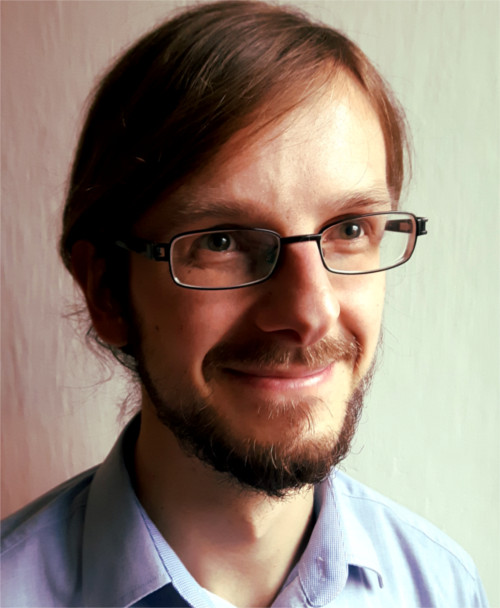
\includegraphics[scale=0.48]{photo.jpg}}\\
%  github: \href{https://github.com/piotr-szachewicz}{https://github.com/piotr-szachewicz}\\
\end{tabular}

%\section{Date of birth}
%18 August 1986
%\\

\section{Education}

\textbf{Poznań University of Technology} (Poland)
	\begin{outerlist}
		\item[] MSc Eng in Computer Science (February 2012 - July 2013)
		\item[] Specialization: Intelligent Decision Support Systems\\
	\end{outerlist}

\textbf{Universitat Roviri i Virgili} (Spain)
	\begin{outerlist}
		\item[] Erasmus exchange (September 2012 - February 2013)\\
	\end{outerlist}
	
\textbf{Poznań University of Technology} (Poland)
	\begin{outerlist}
		\item[] BSc Eng in Computer Science (October 2008 - February 2012)\\
	\end{outerlist}

\textbf{Adam Mickiewicz University, Faculty of Physics} (Poland)

	\begin{outerlist}
		\item[] BSc in Acoustics/Sound Engineering (October 2005 - June 2008)
	\end{outerlist}

\section{Experience}

\textbf{March 2020 - present} -- Spotify -- \textbf{Senior Engineer} (London).
	\begin{outerlist}
		\item[] \textbf{Product:} Content Compliance systems, proactive detection of policy violating content, systems to review flagged content.
		\item[] \textbf{Technologies:} Java, GKE, Salesforce
		\item[] \textbf{Other responsibilities:} driving design discussions with stakeholders and other teams, writing RFCs, interviewing, onboarding new colleagues, helping to organize internal conferences, mentor in an internal Spotify mentoring program, member of a Technical Steering Group.\\
	\end{outerlist}



\textbf{December 2018 - February 2020} -- Spotify -- \textbf{Software Engineer} (London).
	\begin{outerlist}
		\item[] Relocated to London to continue working on the Product Catalog with a newly hired team.\\
	\end{outerlist}

\textbf{July 2017 - November 2018} -- Spotify -- \textbf{Software Engineer} (Stockholm).

	\begin{outerlist}
		\item[] \textbf{Product:} Product Catalog - internal system to configure products and offers launched by Spotify in different markets.
		\item[] \textbf{Technologies:} Python, Java\\
	\end{outerlist}

\textbf{October 2014 - April 2017} -- Sage -- \textbf{Senior Ruby on Rails Developer}\\(Barcelona, Spain).

\begin{outerlist}
  \item[] \textbf{Product:} \href{http://uk.sageone.com/}{Sage Business Cloud Accounting} -- online accounting software.
  \item[] \textbf{Tools:} Ruby on Rails, React.\\\\
\end{outerlist}

\textbf{January 2013 - September 2014} -- Titanis -- \textbf{Python Developer} (Poznań, Poland).

\begin{outerlist}
 \item[] \textbf{Product:} \href{http://neuro-forma.com}{Neuroforma}, neurorehabilitation software with elements of virtual reality.
 \item[] \textbf{Tools:} Python, Django, CoffeeScript.\\
\end{outerlist}

%\pagebreak

%\textbf{July 2011 - September 2011} -- Titanis -- \textbf{C++ Developer}.
%\begin{outerlist}
%  \item Product: Eyetracker, software for a head-mounted eyetracker.
%  \item Tools: C++, openFrameworks, video image processing.
  %\item \url{http://git.nimitz.pl/eyetracker.git}\\
%\end{outerlist}

\textbf{May 2011 - September 2011} -- Alliance Technology -- \textbf{Java EE Developer}.
\begin{outerlist}
  \item[] \textbf{Product:} banking software.
  \item[] \textbf{Tools:} Java EE, Hibernate.\\
\end{outerlist}

\textbf{August 2010 - January 2013} -- Titanis -- \textbf{Java Developer}.
\begin{outerlist}
  \item[] \textbf{Product:} \href{https://github.com/BrainTech/svarog}{Svarog} -- EEG signal viewer, annotator, analyzer and recorder.
  \item[] Tools: Java, Maven, digital signal processing.\\
\end{outerlist}

\textbf{October 2009 - January 2010} -- Adam Mickiewicz University -- \textbf{Teaching Assistant}.
\begin{outerlist}
 \item[] Human-Computer Interaction laboratory practical classes.\\
\end{outerlist}

%\item[] \textbf{2006 - 2009} -- sound engineer in Blue Note Jazz Club, Poznań.

\section{Other projects}

\textbf{March 2012 - November 2013} -- Poznan University of Technology -- publication.
\begin{outerlist} 
  \item[] \textbf{Project:} \href{http://goo.gl/Q9VUsw}{Automatic species counterpoint composition by means of the dominance relation}. Published in \href{http://goo.gl/Q9VUsw}{"Journal of Mathematics and Music"}, 2015.
  \item[] \textbf{Tools:} Java, Python, Latex.\\
\end{outerlist}

\textbf{June 2012 - June 2013} -- Poznan University of Technology -- \textbf{MSc Eng thesis}.
\begin{outerlist}
  \item[] \textbf{Project:} \href{https://github.com/piotr-szachewicz/event-related-desynchronization}{Classification of Motor Imagery for Brain-Computer Interfaces.}
  \item[] \textbf{Tools:} Python, Machine Learning, EEG, DSP.\\
\end{outerlist}

\textbf{September 2011 - January 2012} -- Poznan University of Technology -- \textbf{BSc Eng~thesis}.
\begin{outerlist}
  \item[] \textbf{Project:} developing scholarship module for Sokrates 2 -- a computer system for managing teaching at universities created by the Poznań University of Technology.
  \item[] \textbf{Tools:} Java EE, Maven, Apache CXF, Adobe Flex, Hibernate, Oracle Database.\\
\end{outerlist}



%\section{Conferences/Papers}

%\begin{outerlist}

%\item[] \textbf{2013} -- M. Komosiński, P. Szachewicz, ``Automatic species counterpoint composition using the dominance relation'' (paper; in progress)

%\item[] \textbf{June 2012} -- Concepts-thinking-information, Poznań -- ``Automatic counterpoint composition' (speech).

%\item[] \textbf{December 2009} -- 5th Poznań Cognitive Science Forum (5. Poznańskie Forum Kognitywistyczne) -- ``Computational aesthetics. Methods for automatical aesthetic value evaluation.'' (speech + paper).

%\item[] \textbf{January 2009} -- 4th Poznań Cognitive Science Forum -- ``How to build an artificial artist? Review of approaches to artificial art generation.'' (speech + paper).

%\end{outerlist}

%\section{Skills}

%web-related:
%\begin{outerlist}
% \item CoffeeScript, jQuery, jQuery UI, Django, RESTful WebServices, PHP
%\end{outerlist}

%Java related -- Java, Java Enterprise Edition, JUnit, Maven \\
%databases --- Relational Databases, ORM (Hibernate, Django ORM)
%version control --- Git, Mercurial, Subversion
%other --- Linux, Python, Digital Signal Processing, Electroencephalography, LaTeX, Artificial Intelligence, Machine Learning, Octave, Matlab, OOP, Scrum

% C++, NoSQL, Hadoop, Erlang, C\#

\section{Languages} Polish, English, Spanish

\section{Personal interests} \href{http://sh-ch.band/}{SH-CH} -- instrumental music project

\end{document}

%%%%%%%%%%%%%%%%%%%%%%%%%% End CV Document %%%%%%%%%%%%%%%%%%%%%%%%%%%%%
